\section{干渉計算}

\subsection{干渉計算の概要}

干渉計算は2組の幾何モデルが交差するかを判定しその距離を求める処理である.
主に以下の2つ機能を提供する.
\begin{itemize}
  \item 2つのモデルが交差するかを判定する衝突検出 (collision-check関数)
  \item 2つのモデル間の最短距離を算出する距離計算 (collision-distance関数)
\end{itemize}

irteusでは,他言語インターフェースを介して外部ライブラリを呼び出すことで干渉計算を実行する.
外部ライブラリとして,PQPとBulletの呼び出しが実装されており,デフォルトではPQPが利用される.
以下のように,select-collision-algorithm関数により使用するライブラリを切り替えることができる.
{\baselineskip=10pt
\begin{verbatim}
(select-collision-algorithm *collision-algorithm-pqp*) ;; use PQP
(select-collision-algorithm *collision-algorithm-bullet*) ;; use Bullet
\end{verbatim}
}

個々の外部ライブラリの特徴については以降で詳しく説明する.
他の干渉計算ソフトウェアパッケージについては http://gamma.cs.unc.edu/research/collision/に詳しい.(情報が古い可能性があるので注意.例えばBulletは載っていない.)

\input{irtcollision-func}

\subsubsection{物体形状モデル同士の干渉計算例}
以下は,collision-checkやcollision-distanceを利用して,2つの立方体の衝突検出と距離計算を行い,最近点どうしを結ぶ線分を描画する例である.
干渉が生じているときにcollision-distance関数で得られる最近点は,PQPとBulletで仕様が異なる.詳しくは以降のBulletに関する説明を参照.
{\baselineskip=10pt
\begin{verbatim}
;; Make models
(setq *b0* (make-cube 100 100 100))
(setq *b1* (make-cube 100 100 100))

;; Case 1 : no collision
(send *b0* :newcoords (make-coords :pos #f(100 100 -100)
                                   :rpy (list (deg2rad 10) (deg2rad -20) (deg2rad 30))))
(objects (list *b0* *b1*))
(print (collision-check *b0* *b1*)) ;; Check collision
(let ((ret (collision-distance *b0* *b1*))) ;; Check distance and nearest points
  (print (car ret)) ;; distance
  (send (cadr ret) :draw-on :flush nil :size 20 :color #f(1 0 0)) ;; nearest point on *b0*
  (send (caddr ret) :draw-on :flush nil :size 20 :color #f(1 0 0)) ;; nearest point on *b1*
  (send *irtviewer* :viewer :draw-line (cadr ret) (caddr ret))
  (send *irtviewer* :viewer :viewsurface :flush))

;; Case 2 : collision
(send *b0* :newcoords (make-coords :pos #f(50 50 -50)
                                   :rpy (list (deg2rad 10) (deg2rad -20) (deg2rad 30))))
(objects (list *b0* *b1*))
(print (collision-check *b0* *b1*)) ;; Check collision
(let ((ret (collision-distance *b0* *b1*))) ;; Check distance and nearest points
  (print (car ret)) ;; distance
  ;; In case of collision, nearest points are insignificant values.
  (send (cadr ret) :draw-on :flush nil :size 20 :color #f(1 0 0)) ;; nearest point on *b0*
  (send (caddr ret) :draw-on :flush nil :size 20 :color #f(1 0 0)) ;; nearest point on *b1*
  (send *irtviewer* :viewer :draw-line (cadr ret) (caddr ret))
  (send *irtviewer* :viewer :viewsurface :flush))
\end{verbatim}
}

\begin{figure}[htb]
  \begin{center}
    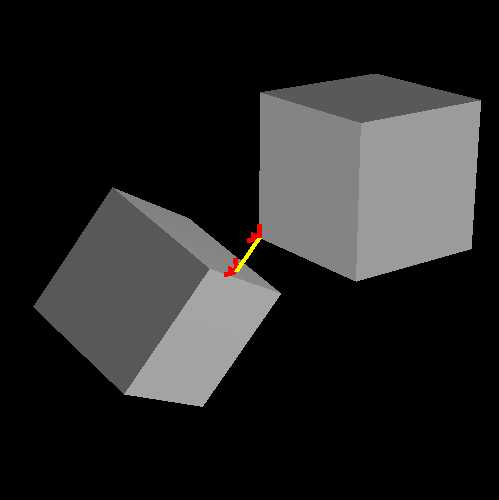
\includegraphics[width=0.50\columnwidth]{fig/collision.jpg}
    \caption{Collision detection}
  \end{center}
\end{figure}

\subsubsection{ロボット動作と干渉計算}
ハンドで物体をつかむ,という動作の静的なシミュレーションを行う場合に手(指)のリンクと対象物体の干渉を調べ,これが起こるところで物体をつかむ動作を停止させるということが出来る.

{\baselineskip=10pt
\begin{verbatim}
(load "irteus/demo/sample-arm-model.l")
(setq *sarm* (instance sarmclass :init))
(send *sarm* :reset-pose)
(setq a 42)
(send *sarm* :move-fingers a)
(setq *target* (make-cube 30 30 30))
(send *target* :translate #f(350 200 400))
(objects (list *sarm* *target*))

(send *sarm* :inverse-kinematics *target* :move-target (send *sarm* :end-coords) :debug-view t)
(while (> a 0)
  (if (collision-check-objects
       (list (send *sarm* :joint-fr :child-link)
             (send *sarm* :joint-fl :child-link))
       (list *target*))
      (return))
  (decf a 0.1)
  (send *irtviewer* :draw-objects)
  (send *sarm* :move-fingers a))
(send *sarm* :end-coords :assoc *target*)

(dotimes (i 100)
  (send *sarm* :joint0 :joint-angle 1 :relative t)
  (send *irtviewer* :draw-objects))
(send *sarm* :end-coords :dissoc *target*)
(dotimes (i 100)
  (send *sarm* :joint0 :joint-angle -1 :relative t)
  (send *irtviewer* :draw-objects))
\end{verbatim}
}

同様の機能が,"irteus/demo/sample-arm-model.l"ファイルの:open-hand,
:close-handというメソッドで提供されている.

\subsection{PQPによる干渉計算}

PQPはノースカロライナ大学のLin氏らのグループにより開発された干渉計算ライブラリである.
PQPソフトウェアパッケージの使い方はirteus/PQP/README.txtに
書いてあり,irteus/PQP/src/PQP.hを読むことで理解できるようになっている.

irteusでPQPを使うためのファイルは
CPQP.C, euspqp.c, pqp.l
からなる.
2つの幾何モデルが衝突してしるか否かを判定するためには,
{\baselineskip=10pt
\begin{verbatim}
(defun pqp-collision-check (model1 model2
				       &optional (flag PQP_FIRST_CONTACT) &key (fat 0) (fat2 nil))
  (let ((m1 (get model1 :pqpmodel))  (m2 (get model2 :pqpmodel))
        (r1 (send model1 :worldrot)) (t1 (send model1 :worldpos))
        (r2 (send model2 :worldrot)) (t2 (send model2 :worldpos)))
    (if (null fat2) (setq fat2 fat))
    (if (null m1) (setq m1 (send model1 :make-pqpmodel :fat fat)))
    (if (null m2) (setq m2 (send model2 :make-pqpmodel :fat fat2)))
    (pqpcollide r1 t1 m1 r2 t2 m2 flag)))
\end{verbatim}
}
を呼び出せば良い.
r1,r1,r2,t1はそれぞれの物体の並進ベクトル,回転行列となり,
(get model1 :pqpmodel)でPQPの幾何モデルへのポインタを参照する.
このポインタは:make-pqpmodelメソッドの中で以下のよう計算される.
{\baselineskip=10pt
\begin{verbatim}
(defmethod cascaded-coords
  (:make-pqpmodel
   (&key (fat 0))
   (let ((m (pqpmakemodel))
         vs v1 v2 v3 (id 0))
     (setf (get self :pqpmodel) m)
     (pqpbeginmodel m)
     (dolist (f (send self :faces))
       (dolist (poly (face-to-triangle-aux f))
         (setq vs (send poly :vertices)
               v1 (send self :inverse-transform-vector (first vs))
               v2 (send self :inverse-transform-vector (second vs))
               v3 (send self :inverse-transform-vector (third vs)))
         (when (not (= fat 0))
           (setq v1 (v+ v1 (scale fat (normalize-vector v1)))
                 v2 (v+ v2 (scale fat (normalize-vector v2)))
                 v3 (v+ v3 (scale fat (normalize-vector v3)))))
         (pqpaddtri m v1 v2 v3 id)
         (incf id)))
     (pqpendmodel m)
     m)))
\end{verbatim}
}
ここでは,まず(pqpmakemodel)が呼び出されている.
pqpmakemodelの中では,euqpqp.cで定義されている,

{\baselineskip=10pt
\begin{verbatim}
pointer PQPMAKEMODEL(register context *ctx, int n, register pointer *argv)
{
    int addr = PQP_MakeModel();
    return makeint(addr);
}
\end{verbatim}
}

が呼び出されており,これは,CPQP.Cの
{\baselineskip=10pt
\begin{verbatim}
PQP\_Model *PQP_MakeModel()
{
    return new PQP_Model();
}
\end{verbatim}
}
が呼ばれている.PQP\_Model()はPQP.hで定義されているものであり,
この様にしてeuslisp内の関数が実際のPQPライブラリの関数に渡されてい
る以降,(pqpbeginmodel m)でPQPの幾何モデルのインスタンスを作成し,
(pqpaddtri m v1 v2 v3 id)として面情報を登録している.

\input{pqp-func}

\subsection{Bulletによる干渉計算}

Bulletは物理演算エンジンであり,その一部として干渉計算機能が提供されている.
irteusでBulletを使うためのファイルは
CBULLET.cpp, eusbullet.c, bullet.l
からなる.
関数内部の呼び出し順序はPQPと同様である.

PQPとBulletの違いとして以下が挙げられる.
\begin{itemize}
  \item 干渉が生じているときにcollision-distanceを呼ぶと,PQPでは,距離として0が返り,最近点として意味のない点が返される.一方Bulletでは,距離として干渉をなくすために動かすべき最短距離(penetration depthと呼ばれる)が返る.また,最近点としては,干渉をなくすための最短距離の両端の点が返される.
  \item PQPは非凸のメッシュモデルをそのまま扱うことができるが,Bulletでは非凸のモデルの凸包を内部で計算しそれを扱っている.
\end{itemize}

\input{bullet-func}
